\documentclass[12pt, a4paper]{article}

\usepackage[fleqn]{amsmath}
\usepackage[margin = 1in]{geometry}

\setlength{\parskip}{\medskipamount}
\setlength{\parindent}{0pt}
\renewcommand{\baselinestretch}{1.2}

\usepackage{graphicx}
\graphicspath{ {/} }

\usepackage{multicol}
%\usepackage{wrapfig}

\usepackage[
backend=bibtex,
style=authoryear,
citestyle=authoryear
]{biblatex}
\addbibresource{refs/refs.bib}

\begin{document}
	
	\title{MultiBiDAF - A Multi-Sentence Reading Comprehension Model}
	\author{Eitan-Hai Mashiah and Noam Barda}
	\maketitle
	
	\begin{multicols}{2}
		
		\section{Introduction}
		
			Machine comprehension is a task of natural language processing wherein the algorithm is presented with a context paragraph and a query, and must answer the query using the information in the paragraph. While this is one of the classical tasks of NLP (\cite{Mccarthy1976}), interest in it has surged in recent years thanks to algorithmic advances (such as recurrent neural networks) and new benchmark datasets such as CNN/daily mail (\cite{Hermann2015}), SQuAD (\cite{Rajpurkar2016}), NewsQA (\cite{Trischler2016}) and MultiRC (\cite{N18-1023}).
			
			Despite its rising popularity, performance in this task remains challenging, and algorithms' capabilities are often below those of young children (\cite{Clark2016}).
			
		\section{Datasets}
		
			We will use two datasets in this project: SQuAD for pre-training and multi-RC as the actual challenge. Both will now be described.
			
			SQuAD, the Standford Question Answering Dataset (\cite{Rajpurkar2016}) was released in 2016. It is a large dataset with over 100,000 questions written by crowd-sourced workers on wikipedia articles.
			
			It has several defining characteristics:
			\begin{enumerate}
				\item A single context paragraph has several questions attached to it.
				\item An answer is always a span of text in the paragraph. This is critical.
				\item There isn't a predetermined list of answers to choose from.
			\end{enumerate}
		
			Version 2.0 of this dataset (\cite{Rajpurkar2018}) also adds questions for which no answer exists in the paragraph, requiring the answering algorithm to also know when to abstain from answering.
			
			Currently, human performance on SQuAD (F1 = 89.452) far surpasses best machine performance (F1 = 74.422), leaving a wide gap for researchers to fill.
			
			MultiRC (\cite{N18-1023}) is a fairly recent addition to machine comprehension datasets. It consists of \char`~ 6000 questions on \char`~ 800 paragraphs from 7 different knowledge domains.
			
			Its defining characteristics are:
			\begin{enumerate}
				\item Several answers are proposed for each question.
				\item Of which one or more can be true.
				\item Answering requires reasoning over several sentences (specifically, 2-4) in the paragraph that are not a single span. This is the most important characteristic of this dataset.
			\end{enumerate}
		
			The dependence on several sentences was created to force the algorithm to better "understand" the context paragraph, and thus allow better generalization.
			
			Again, we see that human performance (F1 = 86.4) is significantly better than existing algorithms (F1 = 66.1), leaving a wide gap to be addressed.
			
		\section{Baseline Model}
		
			Our attempt at improving performance on the MultiRC dataset will use an existing model as the baseline, altering it in ways that should improve its performance when applied to MultiRC. The model we chose for this task is the Bidirectional Attention Flow for Machine Comprehension (BiDAF) model (\cite{Seo2016}). We will begin by describing the model at large, and will then focus on its main novelty, which is as the name suggests, its attention mechanism. See figure 1 for the complete model diagram as originally published.
			
			The layer-wise structure of the BiDAF model is:
			\begin{itemize}
				\item Character-level embedding using a character-level convolutional neural network.
				\item Word embedding layer using pre-trained word embeddings (GLoVe).
				\item A standard bi-directional multilevel LSTM dubbed the contextual embedding layer.
				\item The bi-directional attention layer, to be described in the next paragraph.
				\item Another standard bi-directional multilevel LSTM dubbed the modeling layer.
				\item An output layer with two parts: One for predicting the start token and one for predicting the end token.
			\end{itemize}
		
			More accurately, the first two layers are input to the third layer, which is then input to the attention layer. This entire process, up to the attention layer, is executed separately for the context and the query. The output of the attention layer together with the unattended output from the contextual layer are both passed to the modeling layer, and that is used to predict the outputs.
			
			The novel part of this model is the attention layer. Generally speaking, classic attention mechanisms (\cite{Bahdanau2014}):
			\begin{itemize}
				\item Summarize the entire context paragraph into a single dense vector by weighting the hidden representations of the RNN.
				\item Are dynamic, allowing the attention weights learned in a previous time step to affect the current time step.
				\item Are uni-directional, with the query attending the paragraph.
			\end{itemize}
		
			In the BiDAF model, on the other hand, the attention mechanism:
			\begin{itemize}
				\item Calculates attention for each time step and passes it on to the next layer, preventing early summarization.
				\item Is static, not allowing the attention weights from the previous time-step to affect the current time-step.
				\item Is bi-directional, from context to query and from query to context.
			\end{itemize}
		
			More concretely, the attention mechanism utilizes a T (context length) by J (query length) learnable similary matrix between the context and query words, whereby for each attending (context or query) word, the attended words are weighted using a softmax function based on the corresponding row or column of the similarity matrix, and then summed.
			
			This model has been shown to achieve state-of-the-art results on multiple datasets, including SQuAD and CNN/DailyMail.
			
			The specific implementation we will use is the one in the AllenNLP project (\cite{Gardner2017ADS}). AllenNLP is an open source NLP research library based on pytorch.
		
		\section{Our Model and Training Process}
		
			The two changes we need to make to better match BiDAF to MultiRC are:
			\begin{enumerate}
				\item Change the output layer to predict up to 4 sentences as matches for the query.
				\item Add a mechanism to decide which answers "fit" the chosen sentences sufficiently to be voted as positive.
			\end{enumerate}
			We will elaborate on each in turn.
			
			\subsection{Multiple Sentences}
		
				While the above-described output layer is a good fit for a dataset such as SQuAD, in which the answer is always a single span from the context paragraph, it is not fitting for MultiRC, in which 2-4 sentences participate in the answer.
				
				To handle this setting, we will replace the original output layer by a new output layer with the following changes:
				\begin{itemize}
					\item Instead of predicting one start token and one end token, it will generate a probability distribution over all tokens in the paragraph. 
					\item 2-4 start tokens will then be chosen from the top 4 most probable words, while the cumulative probability of the chosen words does not exceed a threshold hyper-parameter, $ T_s $.
					\item we will change the loss function to be the negative log probabilities of the correct start tokens, $ \sum_i P_i $.
					\item Predicting the end tokens is now unnecessary, as they are by definition the end of the sentences whose start are the chosen words.
				\end{itemize}
			
			\subsection{Multiple Answers}
				
				Identifying the pertinent sentences is not sufficient to decide which answers are right. Those answers must be chosen based on their agreement with the sentences. To do so, the following process will be performed:
				\begin{itemize}
					\item We will train a TF-IDF model on the all sentences and answer options in the training set.
					\item We will calculate a similarity metric between each answer and each chosen sentence using cosine similarity between TF-IDF weighted word counts in the sentences and the answers.
					\item We will take the maximum such metric for each answer among all sentences.
					\item All answers whose maximum similarity exceeds a  threshold hyper-parameter $ T_a $ will be flagged as true.
				\end{itemize}
		
			\subsection{Training}
				As the number of questions in the MultiRC is clearly not sufficient to properly train a complete neural network, even with pretrained word embeddings, we will opt for a multi-stage training process.
				
				\begin{enumerate}
					\item In the first stage, the model will be pre-trained on the SQuAD dataset.
					\item In the second stage, the model will be fine-tuned on the MultiRC dataset.
					\item The thresholds for the sentences ($ T_s $) and the answers ($ T_a $) will be decided using exhaustive grid search using cross-validation.
				\end{enumerate}
				
				Actual training will be done on a Nvidia Tesla P100 GPU on google cloud.
				
				The full code for the model is available on https://github.com/eitanhaimashiah/multibidaf
			
		\section{Results}
		
			We report final results and learning curves both for the relevant sentences found and for the correct answers found.
			
			Following \cite{Rajpurkar2018} , we define $ A(q) $ as the set of correct items and $ \hat{A}(q) $ as the set of selected items. Precision (positive predictive value) is $ \frac{|A(q)| \cap |\hat{A}(q)|}{|\hat{A}(q)|} $ and recall (sensitivity) is $ \frac{|A(q)| \cap |\hat{A}(q)|}{|A(q)|} $.
			
			Then, (macro-average) $ F1_m $ is the harmonic mean of average precision and average recall of all questions, and $ F1_a $ the harmonic mean of sensitivity and recall measured by first "OR"ing all the correct and chosen answers.
			
			The chosen thresholds following cross-validation were $ T_s =  0.6$ and $ T_a = 0.1$
		
			Pre-training on the squad dataset was carried for 20 epochs, with best-epoch performance of $ F1 = 0.77 $. See figure 2 for a complete learning curve.
			
			Training on the MultiRC dataset was carried for 11 epochs (due to early stopping), with eventual best-epoch validation performance of $ F1_m = 0.774$ and $ F1_a = 0.55 $ on the sentences and $ F1_m = 0.59 $ and $ F1_a = 0.58 $ on the answers. See figure 3 for a complete learning curve.
			
			As the MultiRC test set is not publicly available, test (as opposed to validation) results can only be had by sending the model's results to the dataset authors. This process takes a few weeks, and test results were not available in time for submission.
			
		\section{Conclusion}
		
			Our validation result of $ F1_m = 0.59 $ on the answers falls short of the state-of-the-art results of $ F1 = 66.1 $, but not by much. As there is a significant decline in performance between finding the relevant sentences and finding the correct answers, it is possible that a better similarity calculation could achieve better results.
		
			In this project we illustrated that a neural network model, utilizing a bi-directional attention flow mechanism, can achieve good performance on the MultiRC dataset. More specifically, we have shown that BiDAF can be successfully generalized to find several sentences from a given paragraph to answer a given question. To achieve this, the model has to undergo a modification of the output layer and subsequent fine-tuning.
			
			Future directions of research could involve either similar changes to the output layer (e.g. perhaps a NER type layer, tagging spans as belonging to the answer), changes to the similarity calculation between answers and sentences or changes to the actual network.
			
			A change in the similarity calculation could use a network with learnable parameters to estimate the similarity between an answer with the chosen set of sentences, instead of testing sentence-by-sentence as  we did.
		
	\end{multicols}

	\begin{figure*}
		\includegraphics[width=\textwidth,height=10cm]{images/BiDAF.png}
		\caption{BiDAF Model Structure}
	\end{figure*}
	
	\begin{figure*}
		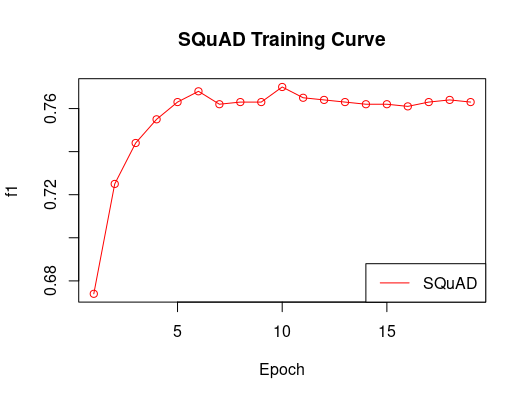
\includegraphics[width=\textwidth,height=10cm]{images/squad.png}
		\caption{SQuAD Pre-Training Learning Curve}
	\end{figure*}
	
	\begin{figure*}
		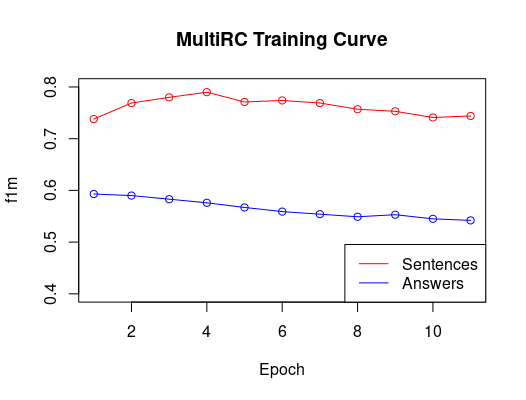
\includegraphics[width=\textwidth,height=10cm]{images/multirc.png}
		\caption{MultiRC Training Learning Curve}
	\end{figure*}

	\printbibliography
	
\end{document}